\chapter{Electric Fields}

\section{Electric Force and Field}

\begin{definition}
    The \vocab{electric charge} is a property of matter that gives rise to electric forces.
\end{definition}

The charge on electrons are designated as negative and that on protons are designated as positive. Like charges repel while unlike charges attract.

The SI unit of electric charge is the coulomb (C), which is defined as ampere second (A s).

\begin{definition}
    A \vocab{charged body} refers to a body that has gained or lost some electrons.
\end{definition}

A body that has gained electrons has a (net) negative charge while one that has lost electrons has a (net) positive charge.

\subsection{Electric Field}

\begin{definition}
    An \vocab{electric field} is a region of space within which an electric charge experiences an electric force.
\end{definition}

An electric field can be represented by directed lines of force. Electric field lines indicate the paths that a small positive test charge would take if it is placed in the field. They always begin on a positive charge and end on a negative charge. Electric field lines do not intersect.

The resultant field of two or more charges can be represented by directed lines which represent the vector sum of their individual fields.

\begin{figure}[H]
    \centering
    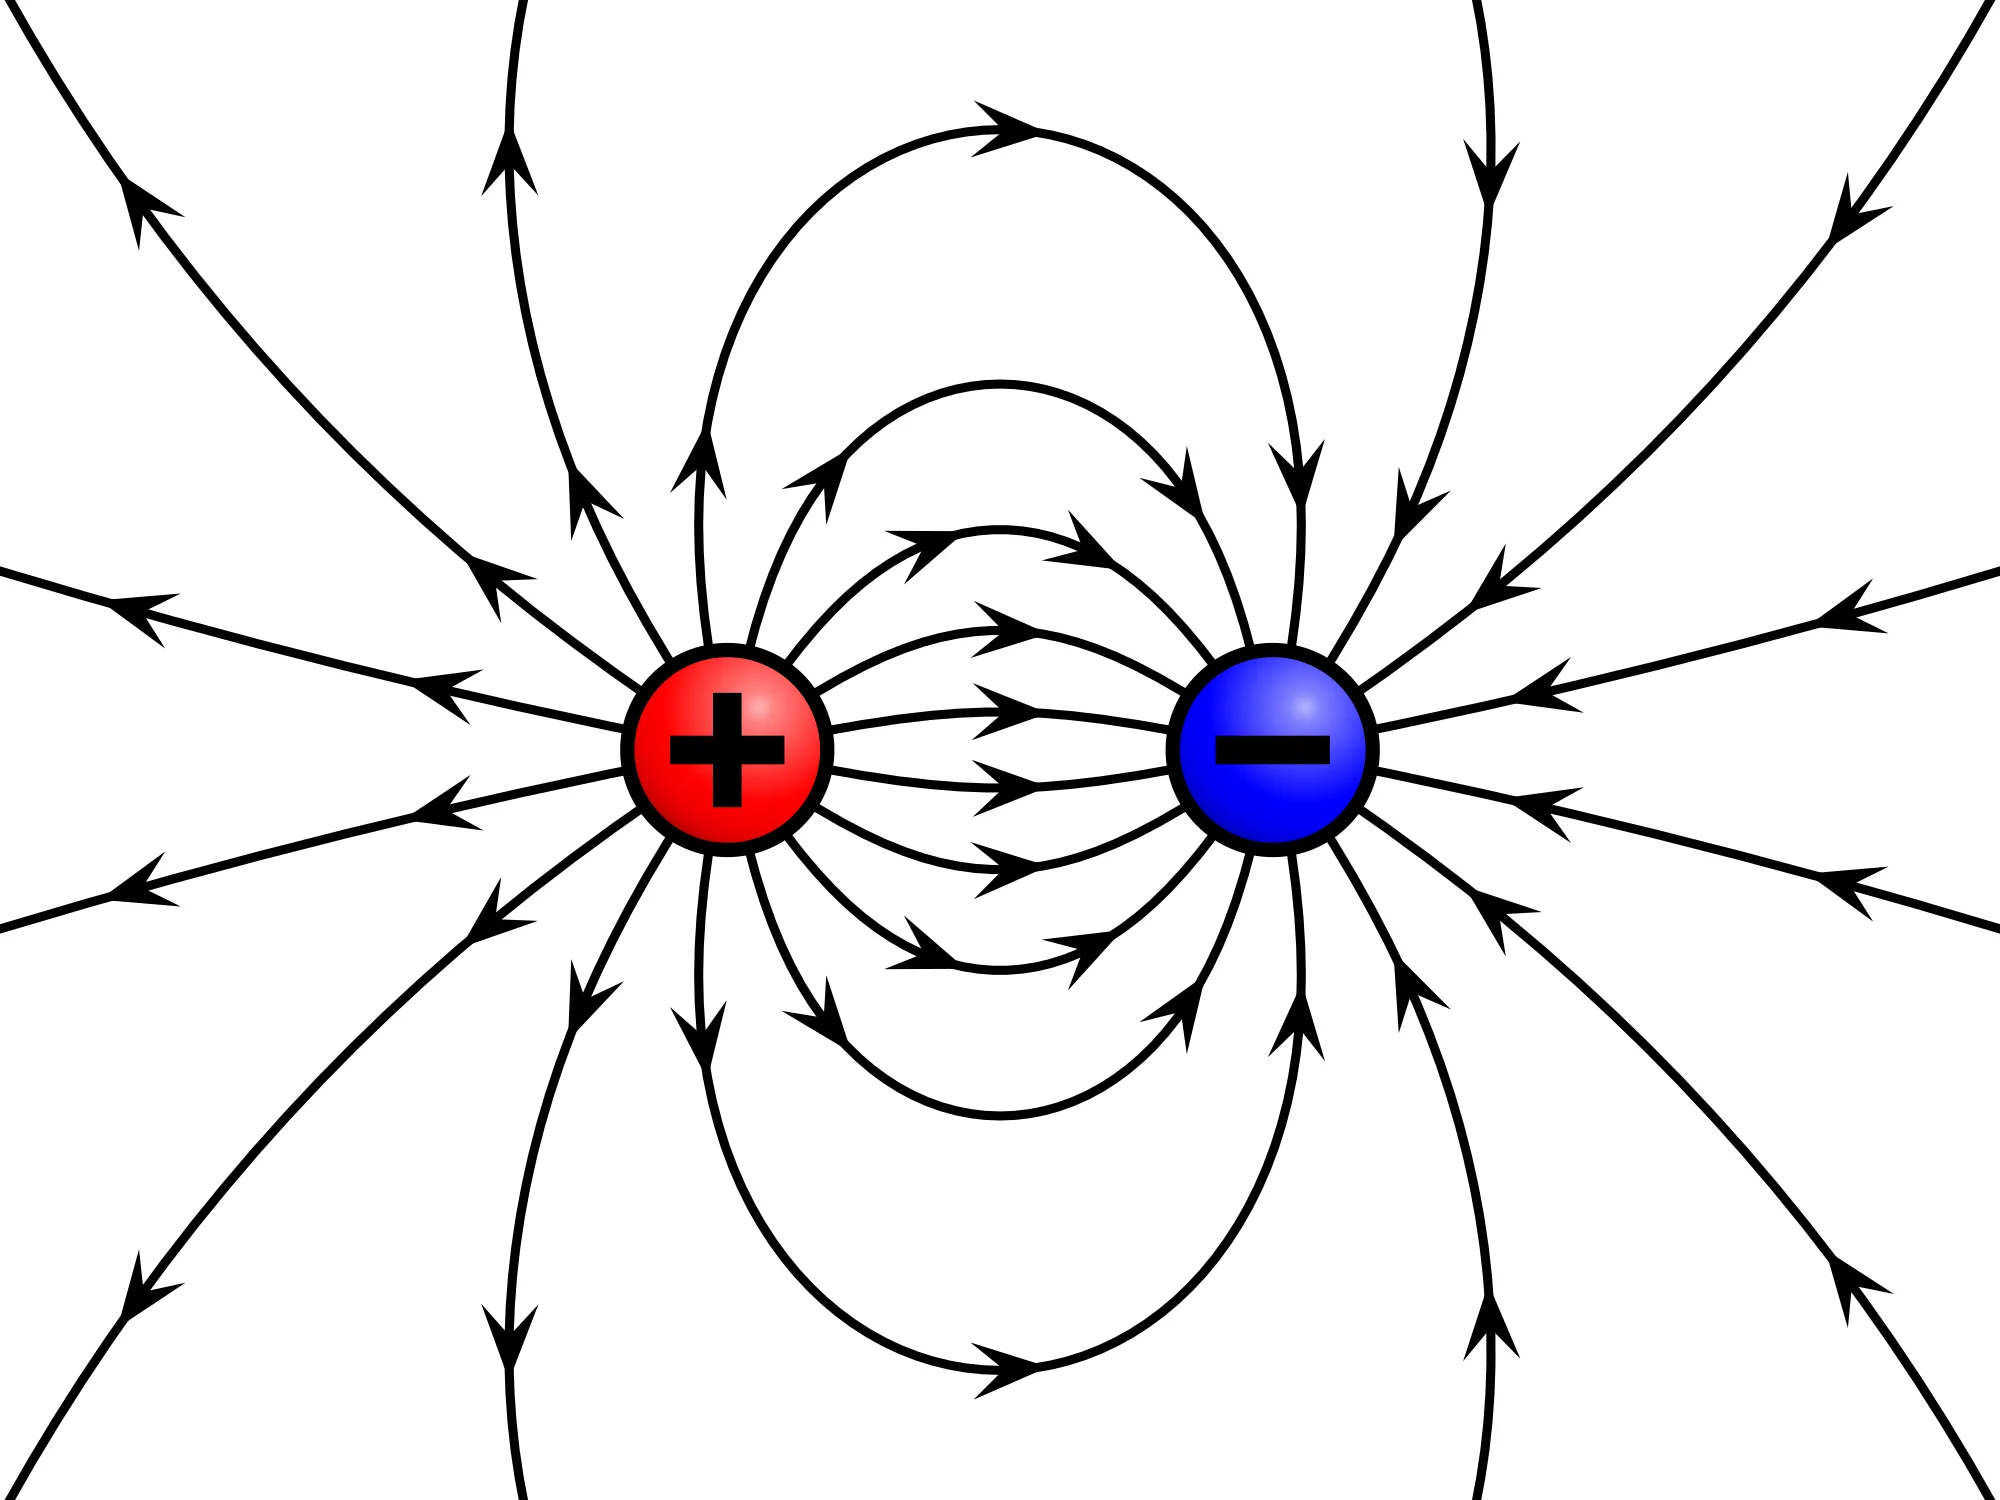
\includegraphics[scale=0.1]{media/Electric Field Line.png}
    \caption{The electric field lines of a field consisting of a positive and a negative charge of equal magnitude.\protect\footnotemark}
\end{figure}
\footnotetext{Source: \url{https://www.faqs.com.pk/what-is-electric-field/}}

On a conducting body, any net charge would reside entirely on its surface. There are no field lines inside the body. Field lines just outside a charged conducting body are always perpendicular to the body's surface.

On an isolated body, there would be more charge per unit area on sharper surfaces and less on flatter surfaces.

\begin{law}[Coulomb's Law]
    Two point charges exert a force on each other that is proportional to the product of their charges and inversely proportional to the square of their separation.
\end{law}

Mathematically, \[F = \frac{Q_1 Q_2}{4\pi \ve_0 r^2},\] where $\ve_0$ ($= 8.85 \times 10^{-12}$ m$^{-3}$ kg$^{-1}$ s$^4$ A$^2$) is the \vocab{permittivity of free space}.

\begin{definition}
    The \vocab{electric field strength} ($E$) at a point in an electric field is the electric force per unit positive charge exerted on a small test charge placed at that point. \[E = \frac{F}{q}.\]
\end{definition}

Electric field strength is a vector quantity. Its SI unit is newton per coulomb (N C$^{-1}$) or volt per metre (V m$^{-1}$).

\begin{proposition}
    The electric field strength $E$ due to a point charge $Q$ at a distance $r$ from the charge is given by \[E = \frac{Q}{4\pi \ve_0 r^2}.\]
\end{proposition}
\begin{proof}
    From Coulomb's law, we see that \[E = \frac{F}{q} = \frac{Q}{4\pi \ve_0 r^2}.\]
\end{proof}

\section{Electric Potential Energy}

\begin{definition}
    The \vocab{electric potential energy} ($U$) at a point is the work done in bringing a small test charge from infinity to that point.
\end{definition}

\begin{proposition}
    In an electric field with point charges $Q_1$, $\dots$, $Q_n$ at distances $r_1$, $\dots$, $r_n$ from a point charge $q$, the electrical potential energy of $q$ is given by 
\end{proposition}
\begin{proof}
    Recall that $F = -\derx{U}{r}$, so \[U_i = -\int_{\infty}^{r_i} F \d r = -\int_{\infty}^{r_i} \frac{Q_i q}{4\pi \ve_0 r^2} \d r = \frac{q}{4\pi \ve_0} \int_{\infty}^{r_i} -\frac{Q_i}{r^2} \d r = \frac{q}{4\pi \ve_0} \frac{Q_i}{r_i}.\] Adding all $n$ contributions together, we get \[U = \frac{q}{4\pi \ve_0} \sum_{i = 1}^n \frac{Q_i}{r_i}\] as desired.
\end{proof}

\begin{definition}
    The \vocab{electric potential} ($V$) at a point is the work done per unit positive charge in bringing a small test charge from infinity to that point. Mathematically, we have \[V = \frac{U}{q}.\]
\end{definition}

Electric potential is scalar quantity. Its SI unit is the volt (V) or joule per coulomb (J C$^{-1}$).

\begin{proposition}
    The electric potential $V$ due to a point charge $Q$ at a distance $r_0$ from the charge is given by \[V = \frac{Q}{4\pi \ve_0 r}.\]
\end{proposition}
\begin{proof}
    By definition, we have \[V = \frac{U}{q} = \frac{Q}{4\pi \ve_0 r}.\]
\end{proof}

Electric potential may be represented by lines of equal potential. The net work done to move a charge between any two points on the same equipotential line is zero.

\begin{figure}[H]
    \centering
    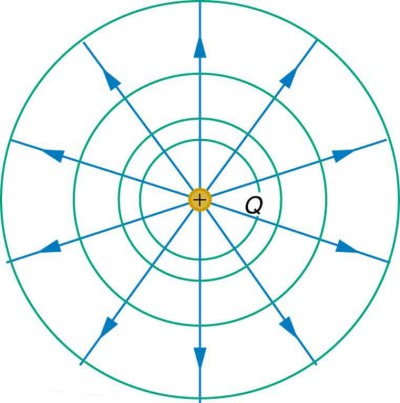
\includegraphics[scale=0.4]{media/Equipotential Lines.jpg}
    \caption{Equipotential lines near a point charge.\protect\footnotemark}
\end{figure}
\footnotetext{Source: \url{https://courses.lumenlearning.com/suny-physics/chapter/19-4-equipotential-lines/}}

Note that equipotential lines are perpendicular to the field lines.

\begin{definition}
    The \vocab{potential gradient} in an electric field is the change in electric potential per unit displacement in the direction of the field. Mathematically, \[\text{potential gradient} = \der{V}{r}.\]
\end{definition}

Potential gradient is a vector quantity. Its SI unit is joules per kilogram per metre (J kg$^{-1}$ m$^{-1}$).

\begin{proposition}
    The electric field strength $E$ at a point is numerically equal but opposite in direction to the potential gradient at that point. Mathematically, \[E = -\der{V}{r}.\]
\end{proposition}
\begin{proof}
    By the definition of $E$ and $V$, we see that \[E = \frac{F}{q} = -\frac1{q} \der{U}{r} = -\der{U/q}{r} = -\der{V}{r}.\]
\end{proof}

The below figure summarizes the relationships between $F$, $U$, $E$ and $V$. Observe the parallels with gravitational fields.

\begin{figure}[H]
    \centering
    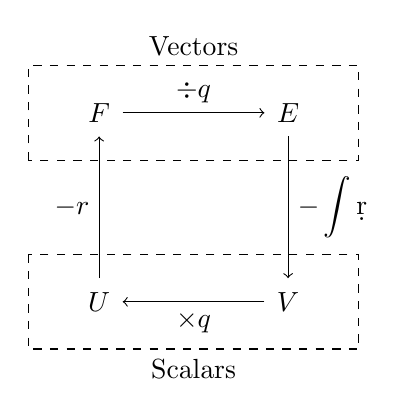
\begin{tikzpicture}[scale=0.6]
        \node at (-2, 2) {$F$};
        \node at (2, 2) {$E$};
        \node at (-2, -2) {$U$};
        \node at (2, -2) {$V$};

        \draw[->] (-1.5, 2) -- (1.5, 2);
        \node[anchor=south] at (0, 2) {$\div q$};

        \draw[->] (1.5, -2) -- (-1.5, -2);
        \node[anchor=north] at (0, -2) {$\times q$};

        \draw[->] (2, 1.5) -- (2, -1.5);
        \node[anchor=west] at (2, 0) {$\displaystyle -\int \d r$};

        \draw[->] (-2, -1.5) -- (-2, 1.5);
        \node[anchor=east] at (-2, 0) {$\displaystyle -\der{}{r}$};

        \draw[dashed] (-3.5, 1) rectangle (3.5, 3);
        \draw[dashed] (-3.5, -1) rectangle (3.5, -3);

        \node[anchor=south] at (0, 3) {Vectors};
        \node[anchor=north] at (0, -3) {Scalars};
    \end{tikzpicture}
    \caption{A summary of electric fields.}
\end{figure}

\section{Uniform Electric Fields}

The electric field between a pair of charged parallel plates with a small separation is almost uniform near the centre. The field becomes more uniform as the plate separation decreases and/or the area of the plates increases.

\begin{proposition}
    The uniform field strength $E$ between a pair of parallel plates with potential difference $V$ and separation $d$ is given by \[E = \frac{V}{d}.\]
\end{proposition}
\begin{proof}
    Observe that \[qV = U = W = Fd = qEd \implies E = \frac{V}{d}.\]
\end{proof}

Within a uniform electric field, where the field strength $E$ is the same at all points, a charged particle will experience a constant electric force in the direction of the field if the charge is negative, and in the opposite direction if it is negative. The motion of charged particles in a uniform electric field is therefore one of uniform acceleration in a direction parallel to the field, and the equations of motion can be used to analyse its trajectory.